\begin{abstract}
A search agent answers a Hindi or Telugu question less accurately than the same question in English. The cause may be the agent's queries (the \emph{query-side gap}) or missing evidence in the user's language (the \emph{evidence-side gap}), and each needs a different fix. We separate them with human-parallel Hindi/English and Telugu/English questions whose answer is in both Wikipedias (287 Hindi, 127 Telugu), a frozen pool of 1.9 million Wikipedia passages served as English-only, Indic-only or both, and a logged, then forced, query language. Four models (three Gemini, one open-weight Qwen3) run the grid under a dense cross-lingual retriever and under BM25. With dense retrieval, the cheapest models lose 9 points on Hindi questions and the stronger Gemini models lose 2--3 (not significant). Changing the query language or pool recovers almost nothing, and with the gold passage in the prompt Hindi is still 4--6 points worse: the residual gap is reading. Under BM25 the Hindi gap is 19--20 points, and dual-language queries recover 9--14. The Hindi and Telugu Wikipedias hold the answer for only 29\% and 24\% of questions; on the uncovered questions a Hindi user reaches 51\% against 60\% for an English user.
\end{abstract}

\section{Introduction}
\label{sec:intro}


Hundreds of millions of people in India now reach the web through chat products backed by search agents: a language model that writes queries, reads the results and answers. When the question is in Hindi, Telugu or Bengali instead of English, the answer is wrong more often. Benchmarks for browsing and deep-research agents report this drop across many languages \citep{a2505_15935,a2608_08775,a2606_15345,a2610_03574}. They do not report \emph{why} it happens, and the cause decides the fix.

Two causes produce the same drop. The first is the agent. It may write a worse query in Hindi than in English, or search in a language where the evidence is not, for example an English query for a fact that only Hindi Wikipedia records. We call this the \textbf{query-side gap}; prompting and training can fix it. The second is the web. Hindi Wikipedia has 2.4\% as many articles as English Wikipedia, Telugu has 1.8\%, and Hindi makes up 0.2\% of Common Crawl pages. If a fact is not written in the user's language, no query in that language will find it. We call this the \textbf{evidence-side gap}; only cross-lingual search or new content can close it. A third gap remains when the model has the right passage and still answers worse in Hindi; we call it the \textbf{integration gap}.

Prior work has measured parts of this problem but not separated the three gaps for a search agent. XBCP translates an English deep-research corpus into twelve languages and measures how much oracle retrieval recovers. Its questions are always in English, the agent's query language is never logged or controlled, and no Indic language is included \citep{a2606_15345}. MarathiWeb studies two web-search models on native Marathi queries and attributes failures to integration by inspection \citep{kale2026marathiweb}. DELTA shows that an apparent preference for English evidence in single-shot RAG partly reflects where the gold evidence lives \citep{a2601_02956}. Where's Waldo shows that, with fixed context, models prefer the query's language when a fact exists in only one Wikipedia edition \citep{a2610_00606}. Section~\ref{sec:related} covers the wider literature.

We build a controlled setup that measures all three gaps (Figure~\ref{fig:schematic}). We fix the question with parallel Indic/English pairs whose evidence exists in both languages. We fix the evidence with a frozen two-language Wikipedia pool that we serve as English-only, Indic-only or both. We log the script of every query under a free policy and then force the query language. We run the grid under a dense cross-lingual retriever and under BM25, because the retriever's language behaviour is part of the query-side gap. Finally, we measure how often the Hindi and Telugu Wikipedias contain each answer, and use this coverage to estimate the accuracy a real user would see.


\begin{figure}[t]
\centering
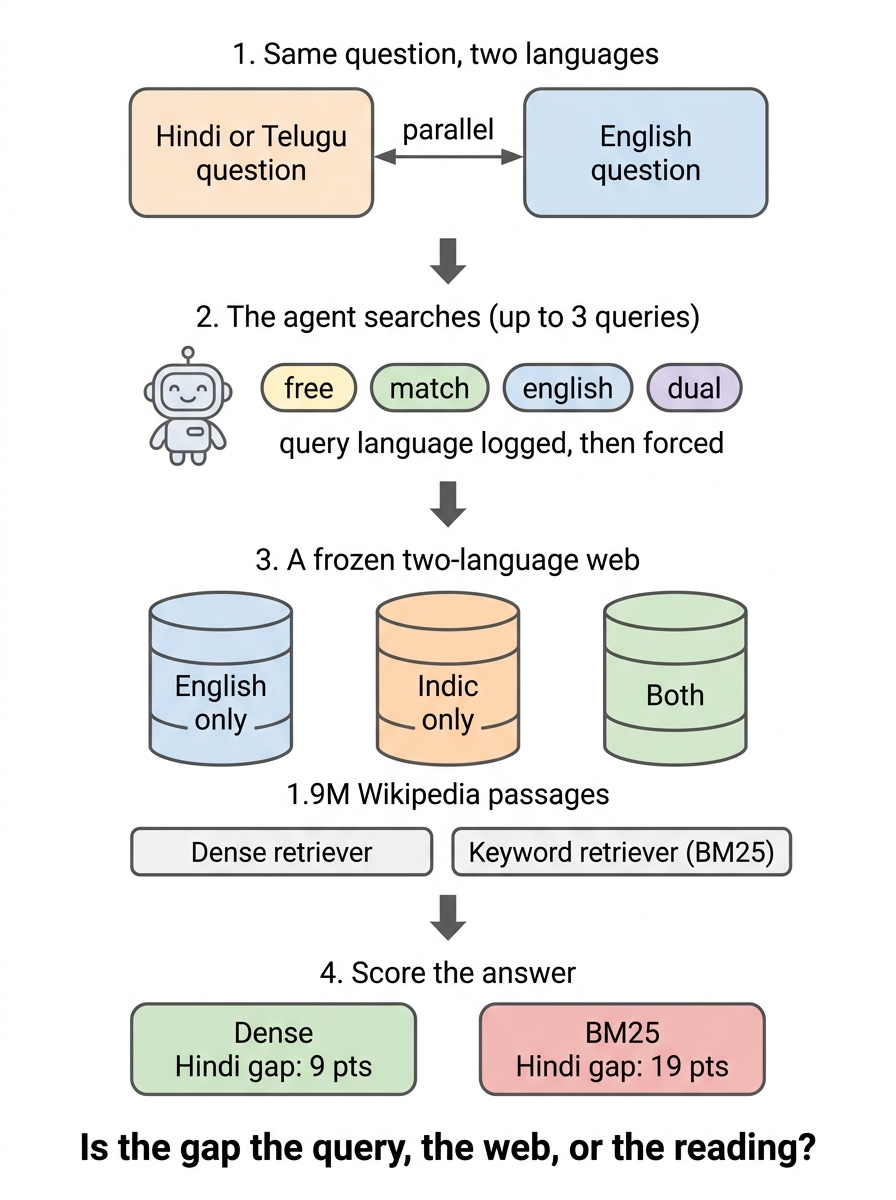
\includegraphics[width=0.8\columnwidth]{assets/fig1_schematic.png}
\caption{Study design. The same question is asked in an Indic language and in English. The agent searches a frozen Wikipedia pool served as English-only, Indic-only or both, under a free or forced query-language policy, with a dense or keyword retriever. The gaps shown are for Gemini 2.5 Flash-Lite, Hindi question, free policy, both pools.}
\label{fig:schematic}
\end{figure}

Our contributions are:
\begin{enumerate}\setlength\itemsep{0pt}
\item \textbf{A controlled setup} that treats the agent's query language as a measured and then manipulated factor, on parallel questions over a frozen pool where the evidence language is served or withheld.
\item \textbf{The retriever as a factor.} With a dense cross-lingual retriever the query-side gap is at most a few points. With BM25 it is 19--20 points for Hindi, and dual-language queries recover 9--14 points.
\item \textbf{A measured coverage term} for the Hindi and Telugu Wikipedias (29\% and 24\%). We also measure the uncovered questions directly instead of extrapolating to them.
\item \textbf{Evidence that the residual gap is reading.} With the gold passage in the prompt, the cheaper models still answer Hindi questions 4--6 points worse; the stronger Gemini models do not.
\end{enumerate}

\section{Related Work}
\label{sec:related}

\paragraph{Agentic search beyond English.} Browsing benchmarks exist for Chinese \citep{a2504_19314}, Korean \citep{a2606_02404,a2606_27595}, and thirteen natively authored languages without an Indic one \citep{a2610_03574}. BrowseComp-Plus fixed the corpus so that retrievers can be swapped \citep{a2508_06600}, and XBCP translated it into twelve languages \citep{a2606_15345}. Multilingual GAIA variants score 47.4\% in English against 35.8\% in other languages and place Hindi among the weakest at every model size \citep{a2505_15935,a2608_08775}; part of that gap may be translation artefact \citep{a2604_24929}. English-only studies split agent failures into retrieval and use of the retrieved text \citep{a2608_01913,a2608_05212,a2609_08094}. The MAST shared task runs Indic queries over an English-only corpus \citep{mast2026}, so the evidence-side gap is zero by design. None of these logs or forces the agent's query language for an Indic user, or varies where the evidence lives.

\paragraph{Language preference in multilingual retrieval.} Retrievers and generators favour high-resource and query-language passages \citep{a2502_11175,a2604_20199,a2605_07249,a2509_13930}, and models write tool arguments in the wrong language, Hindi included \citep{a2601_05366}. DELTA corrects for where gold evidence exists statistically \citep{a2601_02956}; we control it experimentally. Studies disagree on whether translating the query helps \citep{a2504_03616,a2510_23070,a2507_22923}; the sign depends on where the documents are \citep{a2507_07543}. XRAG ran a controlled query-language ablation on a live engine \citep{a2505_10089}, and CORAL lets an agent pick the corpus language but reports only end accuracy \citep{a2604_25676}. Dense multilingual retrievers match across languages where lexical matching cannot \citep{a2511_19324,a2402_03216}, which is why we treat the retriever as a factor.

\paragraph{Indic resources and knowledge gaps.} Parallel Indic questions come from IndicGenBench \citep{a2404_16816}, built on TyDi XOR \citep{a2010_11856,clark2020tydi}, and from MLQA \citep{a1910_07475}. India-centric closed-book sets include IndicQuest, MILU and MultiLoKo \citep{a2608_15535,a2504_20022,a2411_02538,a2504_10356}; Indic retrieval resources include MIRACL, IndicIRSuite and Hindi-BEIR \citep{a2210_09984,a2312_09508,a2408_09437}. Factual recall depends on language and script \citep{a2010_06189,a2406_16135,a2510_15551}, and India-centric facts are answered better in English \citep{a2504_20022,a2605_29637}. ECLeKTic and Where's Waldo build questions whose evidence exists in one Wikipedia edition only \citep{a2502_21228,a2610_00606}, the closed-book analogue of our evidence manipulation. Wikipedia's coverage asymmetry has been documented since \citet{hecht2010tower}. The supplementary material compares our design with each close neighbour.

\section{Experimental Setup}
\label{sec:setup}

\subsection{Questions}
\label{sec:questions}
\textbf{XorQA-In} \citep{a2404_16816} provides 539 test questions per language, human-translated from English TyDi XOR questions \citep{a2010_11856}, each with the English paragraph that answers it. For each item we found the Hindi or Telugu counterpart of the English source article through Wikidata sitelinks and checked whether it states the answer. We used string match, then two independent LLM reads that had to quote a sentence found verbatim in the article, and a 50-item manual audit (supplementary material). An item enters the controlled grid only when both reads agree: 157 Hindi and 127 Telugu items. \textbf{MLQA} \citep{a1910_07475} adds 130 self-contained Hindi questions with naturally parallel Hindi and English paragraphs, giving 287 Hindi items in total. A further 120 natively written \textbf{TyDi XOR} Telugu questions test whether translation drives the results \citep{a2604_24929}.

\subsection{Evidence pools and retrievers}
\label{sec:pool}
All pools come from the October 2026 \texttt{wikipedia-monthly} snapshot \citep{wikipediamonthly2026}: the complete Hindi Wikipedia (353{,}075 chunks), the complete Telugu Wikipedia (518{,}524 chunks), and a 1.8\% sample of English Wikipedia (1{,}058{,}175 chunks) plus the English article behind every item. Chunks are about 900 characters with the title prefixed. The agent's one tool, \texttt{search(query)}, returns the top five chunks from the pool being served: English-only, Indic-only, or both. We use two retrievers: BM25 \citep{robertson2009bm25} over Unicode word tokens, and bge-m3 dense embeddings \citep{a2402_03216} with exact inner-product search. With the question itself as the query, BM25 put the gold chunk in the top five for 50\% of English questions but only 8\% of Hindi and 7\% of Telugu ones, because two Devanagari spellings of the same name (``Oregan'' and ``Oregon'' when transliterated) do not match as tokens. bge-m3 reached 70\% for both Indic languages.

\subsection{Agent and query policies}
\label{sec:agent}
The agent is a fixed ReAct loop \citep{a2210_03629} with native tool calling: at most three searches, then a short answer in the question's language, at temperature 0. The policies differ by one sentence in the system prompt: none (\textbf{free}), ``write every query in [the question's language]'' (\textbf{match}), ``write every query in English'' (\textbf{english}), or ``search once in each language'' (\textbf{dual}). For every call we log the query's dominant script and whether a gold chunk was retrieved. The full prompts are in the supplementary material.

The design crosses question language (English or Indic), policy (four levels) and served pool (three levels) into 19 cells. Three extra arms isolate specific gaps: \textbf{closed-book} (no tool) measures what the model already knows; \textbf{oracle} (gold passage in the prompt) measures the integration gap; and a \textbf{repeat battery} (30 items $\times$ 5 runs) measures run-to-run noise.

\subsection{Models}
\label{sec:models}
Table~\ref{tab:models} lists the four models. Three are Gemini models accessed through OpenRouter; Qwen3-30B-A3B-Instruct-2507 is open-weight and served with vLLM on a rented GPU. A guardrail on the API account blocked other closed model families during the study.

\begin{table}[t]
\centering\small
\setlength{\tabcolsep}{4pt}
\begin{tabular}{@{}llrr@{}}
\toprule
Model & Access & Hi & Te \\
\midrule
Gemini 2.5 Flash-Lite & API & 287 & 127 \\
Gemini 3.1 Flash-Lite & API & 100 & 100 \\
Gemini 3.6 Flash & API & 50 & 50 \\
Qwen3-30B-A3B & open weights & 287 & 127 \\
\bottomrule
\end{tabular}
\caption{Models and number of items per language. Gemini 2.5 Flash-Lite and Qwen3 run the full grid under both retrievers plus all arms; Gemini 3.1 Flash-Lite runs the dense grid; Gemini 3.6 Flash runs the headline cells.}
\label{tab:models}
\end{table}

\subsection{Scoring and statistics}
\label{sec:stats}
An answer is correct if it matches a gold alias in either script after normalisation. Otherwise a judge model outside the grid (Gemini 2.5 Flash) labels it correct, wrong or abstain; a hand audit of 40 judged answers agreed with every label (supplementary material). Every contrast is a paired within-item difference with a sign-flip permutation test and a 95\% item-bootstrap interval \citep{efron1994bootstrap}. All $p$-values form one Benjamini--Hochberg family of 144 tests \citep{benjamini1995bh}. The repeat battery changed the verdict on 1 of 30 Hindi items and 0 of 30 Telugu items, so we do not interpret differences below about two points.

To estimate the accuracy a real user would see, we weight the controlled accuracies by coverage, the share of questions whose Indic Wikipedia article states the answer. This is the law of total probability \citep{ross2014probability}:
\begin{equation}
\begin{split}
\mathrm{Acc}_L ={}& \mathrm{Cov}_L \cdot \mathrm{Acc}(L \mid \text{in } L)\\
&+ (1-\mathrm{Cov}_L)\cdot \mathrm{Acc}(L \mid \text{en only}).
\end{split}
\label{eq:decomp}
\end{equation}

\section{Results}
\label{sec:results}

\subsection{Query language under the free policy}
\label{sec:results-drift}
Given a Hindi question, the models write 18--57\% of their queries in English: Gemini 2.5 Flash-Lite 30--33\%, Gemini 3.1 Flash-Lite 31--38\%, Gemini 3.6 Flash 45--57\% and Qwen 18--19\%. For Telugu questions all models use English more often (43--48\%). The share barely changes with the served pool, so the agents do not notice when an English-only pool returns no Hindi text.

\subsection{The gap under dense retrieval}
\label{sec:results-qg}
Table~\ref{tab:main} gives the main contrasts. With evidence in both languages, the Hindi question costs Gemini 2.5 Flash-Lite 9.4 points and Qwen 9.1 points; both survive correction. Gemini 3.1 Flash-Lite and 3.6 Flash lose 3.0 and 2.0 points, with intervals that include zero. No Telugu gap is significant. The gap belongs to the cheaper models, not to the languages.

Where the gap exists, changing the query language does not close it. For Gemini 2.5 Flash-Lite, matched, dual and English-only queries change Hindi accuracy by $+0.7$, $+1.8$ and $+4.5$ points; none survives correction. The gold passage is already in the top five for 79\% of free-policy episodes, so there is little retrieval left to recover. The served pool also makes no difference: the Hindi question scores within one point on English-only and both pools, because bge-m3 finds the English passage for a Hindi query. Figure~\ref{fig:fig3} shows every policy and pool.

\begin{table*}[t]
\centering\small
\setlength{\tabcolsep}{4pt}
\begin{tabular}{@{}lcccc@{}}
\toprule
Contrast (points), Hindi & Gemini 2.5 FL & Gemini 3.1 FL & Gemini 3.6 F & Qwen3-30B \\
\midrule
Total gap, dense (English minus Hindi question) & \textbf{+9.4} [4.5, 14.3] & +3.0 [$-$2.0, 8.0] & +2.0 [$-$4.0, 8.0] & \textbf{+9.1} [3.8, 14.6] \\
\quad recovered by dual queries & +1.8 [$-$3.2, 6.8] & +1.0 [$-$4.0, 6.0] & +0.0 [$-$6.0, 6.0] & +4.5 [0.7, 8.4] \\
\quad recovered by English queries & +4.5 [0.0, 9.1] & +2.0 [$-$3.0, 7.0] & +6.0 [0.0, 14.0] & $-$1.4 [$-$6.3, 3.5] \\
Evidence-side: both minus English-only pool & $-$0.7 [$-$5.6, 3.8] & $-$2.0 [$-$7.0, 3.0] & +0.0 [$-$6.0, 6.0] & +5.6 [1.0, 10.5] \\
Integration gap (gold passage in prompt) & \textbf{+6.3} [2.8, 9.8] & $-$2.0 [$-$6.0, 2.0] & $-$2.0 [$-$10.0, 4.0] & +4.2 [0.7, 7.7] \\
Closed-book gap & +3.1 [$-$1.0, 7.7] & +3.0 [$-$4.0, 10.0] & +2.0 [$-$4.0, 8.0] & \textbf{+12.9} [7.3, 18.5] \\
\midrule
Total gap, BM25 & \textbf{+18.9} [12.9, 24.8] & -- & -- & \textbf{+19.5} [13.6, 25.8] \\
\quad recovered by dual queries, BM25 & \textbf{+9.3} [3.9, 14.6] & -- & -- & \textbf{+13.6} [8.4, 18.8] \\
Hindi question, BM25 minus dense & \textbf{$-$15.7} [$-$21.3, $-$10.1] & -- & -- & \textbf{$-$16.0} [$-$21.6, $-$10.5] \\
\bottomrule
\end{tabular}
\caption{Main paired contrasts for Hindi questions (free policy, both pools unless stated), with 95\% item-bootstrap intervals. \textbf{Bold}: survives Benjamini--Hochberg correction over 144 tests. FL = Flash-Lite, F = Flash. Telugu and all other contrasts are in the supplementary material.}
\label{tab:main}
\end{table*}

\begin{figure*}[t]
\centering
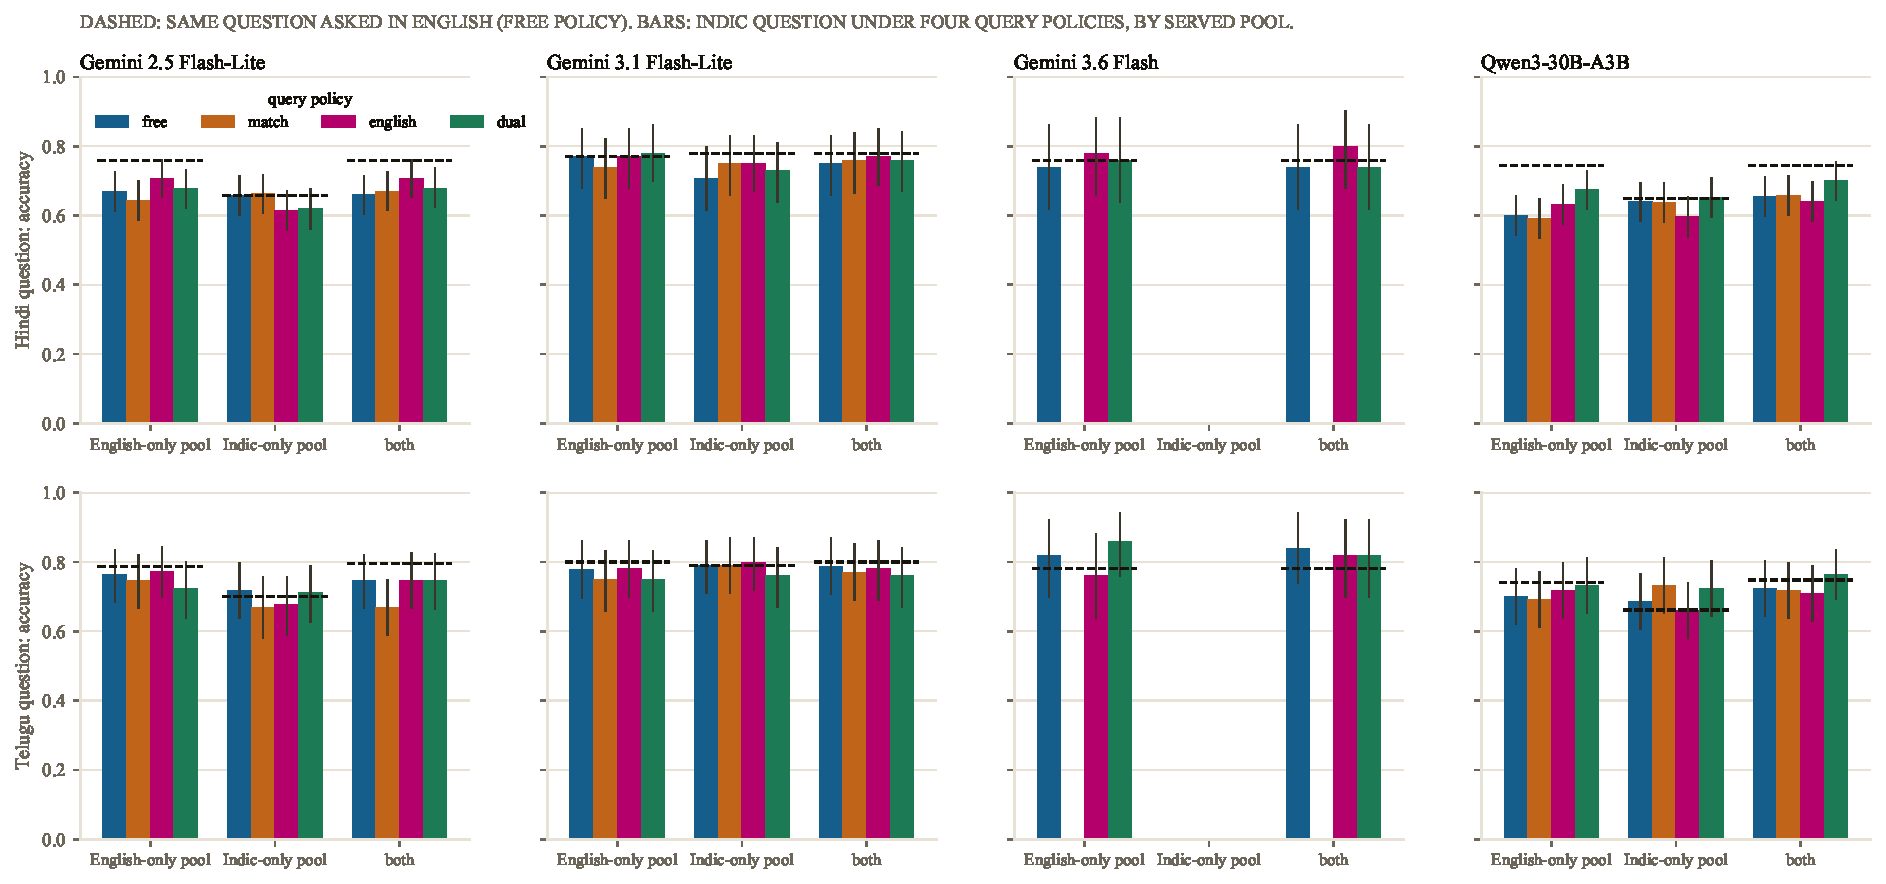
\includegraphics[width=0.78\textwidth]{assets/fig3_policy_by_pool.pdf}
\caption{Accuracy of the Indic question under four query policies and three served pools (dense retriever), with 95\% intervals. The dashed line is the English question under the free policy. Top row Hindi, bottom row Telugu.}
\label{fig:fig3}
\end{figure*}

\subsection{The gap under keyword retrieval}
\label{sec:results-bm25}
BM25 gives the opposite result on the same items. The Hindi question now costs 18.9 points for Gemini 2.5 Flash-Lite and 19.5 for Qwen, and scores about 16 points below the same question under dense retrieval (all survive). Here the query language matters. Dual queries recover 9.3 and 13.6 points (both survive), and English-only queries on the English-only pool reach 62.7\% against 43.4\% for the free policy. The gold passage reaches the top five in 40\% of free-policy episodes under BM25 against 79\% under dense retrieval, and the agent abstains in 23--39\% of BM25 episodes. The query-side gap is large when the search engine matches words in one language and nearly absent when it matches meaning across languages.

\subsection{When searching in English helps and hurts}
\label{sec:results-interaction}
For Gemini 2.5 Flash-Lite on Hindi questions, English queries beat matched-language queries by 6.3 points on the English-only pool and lose 4.9 points on the Hindi-only pool. The interaction is 11.2 points [4.2, 18.2] and survives correction. The effect does not appear for Telugu or for Gemini 3.1 Flash-Lite. This reproduces, for one model and language, the sign flip that earlier query-translation studies disagreed about \citep{a2507_07543,a2504_03616}: the query language mainly decides which pool the agent can read.

\subsection{Coverage and expected user accuracy}
\label{sec:results-decomp}
The linked Hindi article exists for 67.5\% of the 539 XorQA questions and states the answer for 29.1\% [25.2, 33.0]. For Telugu the figures are 52.5\% and 23.6\% [20.0, 27.1]. Table~\ref{tab:decomp} combines coverage with the controlled cells through Eq.~\ref{eq:decomp}.

Extrapolating the covered items gives a Hindi user of Gemini 2.5 Flash-Lite 66.7\% against 75.8\% for an English user under dense retrieval. Under BM25, the Hindi user gets 45.4\% against 71.4\%, and telling the agent to search in English lifts this to 62.9\%. The extrapolation assumes uncovered questions are as easy as covered ones, so we tested it on all 382 uncovered Hindi questions. They are harder for everyone: the English question scores 53.4\% on them against 75.8\% on covered items. The measured expected accuracy is 51.4\% for the Hindi user against 60.5\% for the English user. The extrapolation overstates both users by 15--19 points, but the 9-point gap between them holds. On uncovered questions, serving the Hindi pool alongside English costs 5.8 points (survives): Hindi articles on the topic that lack the fact push the English passage that has it out of the top five.

\begin{table}[t]
\centering\small
\setlength{\tabcolsep}{4pt}
\begin{tabular}{@{}lrrrr@{}}
\toprule
& \multicolumn{3}{c}{Indic user, policy} & English \\
\cmidrule(lr){2-4}
Model, language & free & dual & english & user \\
\midrule
G2.5 FL, Hi & 66.7 & 67.9 & \textbf{70.7} & 75.8 \\
\quad measured & \textbf{51.4} & 50.4 & -- & 60.5 \\
\quad BM25 & 45.4 & 58.4 & \textbf{62.9} & 71.4 \\
G2.5 FL, Te & 76.0 & 72.9 & \textbf{76.6} & 78.7 \\
\quad measured & \textbf{56.8} & 52.7 & -- & 60.1 \\
\quad BM25 & 49.9 & 55.9 & \textbf{67.1} & 66.9 \\
G3.1 FL, Hi & 76.4 & \textbf{77.4} & 77.0 & 77.0 \\
G3.1 FL, Te & \textbf{78.0} & 75.2 & \textbf{78.0} & 80.0 \\
G3.6 F, Hi & 74.0 & 75.4 & \textbf{78.6} & 76.0 \\
G3.6 F, Te & 82.5 & \textbf{85.1} & 77.4 & 78.0 \\
Qwen3, Hi & 61.6 & \textbf{68.3} & 63.4 & 74.6 \\
\quad BM25 & 43.3 & \textbf{59.9} & -- & 69.7 \\
Qwen3, Te & 70.6 & \textbf{74.0} & 71.5 & 74.0 \\
\quad BM25 & 56.6 & \textbf{64.8} & -- & 68.5 \\
\bottomrule
\end{tabular}
\caption{Expected accuracy (\%) for a real user from Eq.~\ref{eq:decomp}, with coverage 29.1\% (Hindi) and 23.6\% (Telugu). Dense retriever unless marked BM25. ``Measured'' rows replace the extrapolated uncovered term with a direct run on the uncovered items. \textbf{Bold}: best query policy for the Indic user in each row.}
\label{tab:decomp}
\end{table}

\subsection{The residual gap is reading}
\label{sec:results-retriever}
With the gold English passage in the prompt, Gemini 2.5 Flash-Lite still answers the Hindi question 6.3 points worse than the English one (survives), and Qwen 4.2 points worse. Given the Hindi question, Gemini 2.5 Flash-Lite answers correctly from the English passage 80.5\% of the time and from the Hindi passage 72.8\%: it reads English evidence better even for a Hindi question. The two stronger Gemini models read as well in Hindi as in English (integration gaps of $-2.0$ points). Closed-book, the models already know many of these facts (57.8--70.0\% for Hindi questions), but 77\% of correct agent answers from Gemini 2.5 Flash-Lite had a gold chunk in the trajectory. The natively written Telugu questions are harder (60.0\% against 74.8\%), but the agent behaves the same way on them: 44\% English queries and no gain from dual queries. Qwen differs from Gemini in one respect: its closed-book Hindi accuracy is 12.9 points below English, so it depends more on retrieval.

\section{Discussion}
\label{sec:discussion}

\paragraph{Comparison with prior findings.} XBCP found retrieval to be a larger loss than integration for deep-research agents over a translated corpus \citep{a2606_15345}. Our BM25 results agree. Our dense-retrieval results do not: with a cross-lingual retriever, retrieval is close to solved and the remaining loss is integration. This is consistent with MarathiWeb's conclusion from inspection that failures come from integration ``rather than missing sources'' \citep{kale2026marathiweb}, which we now measure under controlled conditions. DELTA's point that gold-evidence location confounds language preference \citep{a2601_02956} holds for agents too: the English-query benefit in Section~\ref{sec:results-interaction} reverses when the evidence is only in Hindi.

\paragraph{What a product team should do.} The right fix depends on the search engine. If the engine behind the agent matches words in one language, translate or duplicate the query into English; this recovers about half the Hindi gap. If the engine is cross-lingual, the query language is not the problem, and the remaining gap comes from the model's reading of Indic text, which a stronger model closes. In both cases agents do not adapt on their own: they keep the same mix of query languages whatever the pool returns.

\paragraph{Pre-registered predictions.} We recorded six directional predictions before the first grid call. D3 and D5 held. D1 failed: it predicted that agents would write most queries in English, which held for only one model and pool. D4 held in its first half (coverage below one half) and failed in its second. D2 and D6 split by model.

\section{Conclusion}
\label{sec:conclusion}
We separated the query-side, evidence-side and integration gaps for search agents answering Hindi and Telugu questions. The answer depends on the retriever. With dense cross-lingual retrieval, neither the query nor the web explains the Indic user's deficit: the remaining 2--9 points come from the model reading the evidence, and the strongest models show no gap. With keyword retrieval, the query language decides the outcome: the Hindi question costs 19--20 points and dual-language queries recover about half of that. The facts that Indic Wikipedia lacks are also harder for everyone, and measuring them directly lowers both users' accuracy by 15--19 points while leaving the gap unchanged.

\paragraph{Future work.} Three extensions follow directly. First, more languages, starting with Bengali and Tamil, and natively written questions at scale. Second, a live-web arm with a commercial search engine, to test whether its behaviour resembles our dense or our BM25 condition. Third, training or prompting agents to choose the query language from the results they get back, since none of the models tested did so.

\section*{Limitations}
\label{sec:limits}
Wikipedia is not the web. Our English pool is a 1.8\% sample plus the articles behind each item, so it has fewer near-topic distractors than a real engine would return. We study two Indic languages. The XorQA questions are human translations of English questions; the natively written Telugu subset checks but does not remove this concern. Coverage relies on string match and two LLM reads with a 50-item audit; the audit found the first read too generous, so the reported figure is conservative. The closed-model arm is Gemini only, because an account guardrail blocked other providers, and the open-weight arm is one model. The judge is a Gemini model; string match decides 41\% of items and the hand audit bounds the rest.

\section*{Ethical Considerations}
We use only public Wikipedia text (CC BY-SA) and public benchmark questions. Models were queried through public APIs or run as open weights on our own GPU. No deployed search product was probed and no human subjects were involved. The pools can be rebuilt from the public snapshot with our scripts.

\section*{Use of AI Assistants}
We used AI tools at several stages of this work, and the authors checked all outputs. Claude (Anthropic) helped write the experiment code and analysis scripts and helped draft and edit the paper text. Figure~\ref{fig:schematic} was generated with a Gemini image model (Nano Banana) from a text description of our pipeline, and we checked every label against the design; all data figures are plotted from our results. LLMs are also part of the experimental setup: four models are the agents under study, Gemini models perform the two coverage reads, and Gemini 2.5 Flash judges answers that string matching cannot decide (Section~\ref{sec:stats}).
